% Native editable composition from one verified, unchanged IDE capture.
\begin{figure}[htbp]
\centering
\sbox0{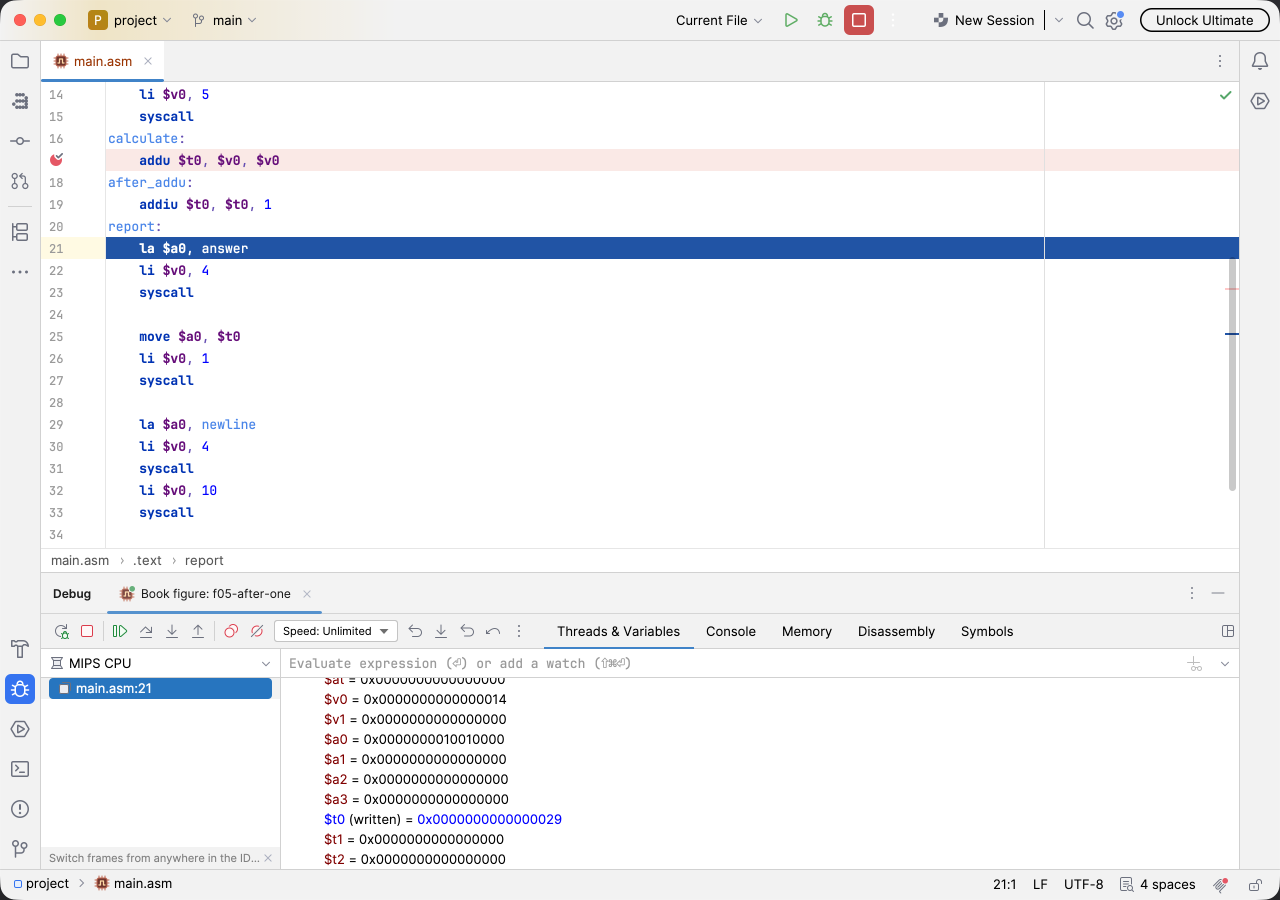
\includegraphics[artifact]{book/captures/001-console-calculation/f05-after-one/raw.png}}
\edef\MARSconsoleafteronesourceLeft{\the\dimexpr0.036718750\wd0\relax}
\edef\MARSconsoleafteronesourceBottom{\the\dimexpr0.707777778\ht0\relax}
\edef\MARSconsoleafteronesourceRight{\the\dimexpr0.611718750\wd0\relax}
\edef\MARSconsoleafteronesourceTop{\the\dimexpr0.236666667\ht0\relax}
\edef\MARSconsoleafteronevalueLeft{\the\dimexpr0.246093750\wd0\relax}
\edef\MARSconsoleafteronevalueBottom{\the\dimexpr0.075555556\ht0\relax}
\edef\MARSconsoleafteronevalueRight{\the\dimexpr0.554687500\wd0\relax}
\edef\MARSconsoleafteronevalueTop{\the\dimexpr0.895555556\ht0\relax}
\begin{tikzpicture}[alt={Two annotated Debug details after addiu. The blue source line at report is la a0 answer, which begins preparing the output message address. Register t0 is hexadecimal 0000000000000029, decimal 41. The arithmetic is complete and the answer has not yet been printed.}]
\node[anchor=north west,inner sep=0,font=\small\bfseries] (source-title) at (6mm,0) {Execution has reached the reporting sequence};
\node[anchor=north west,inner sep=0] (source) at ([yshift=-1mm]source-title.south west) {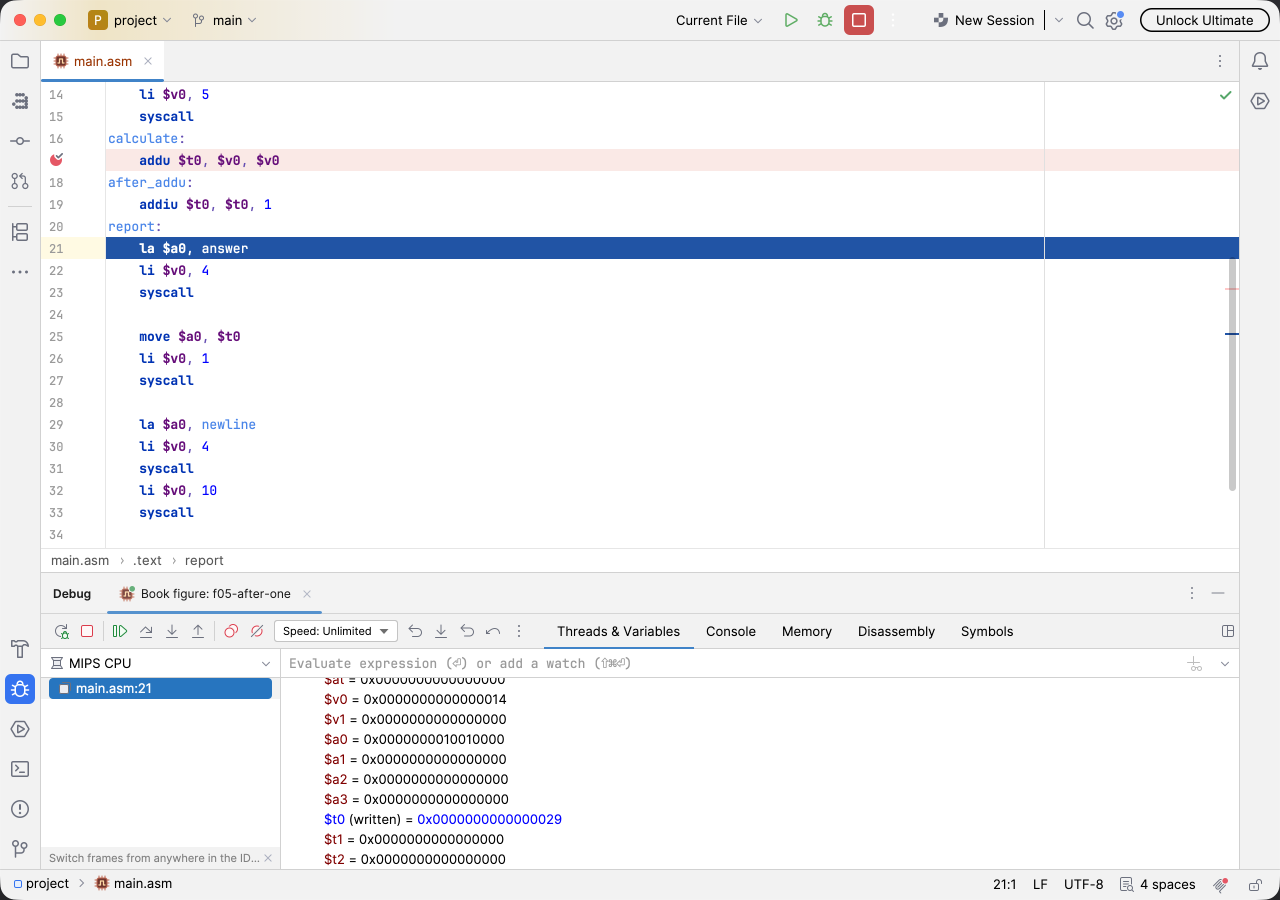
\includegraphics[width=0.7\linewidth,artifact,trim={\MARSconsoleafteronesourceLeft{} \MARSconsoleafteronesourceBottom{} \MARSconsoleafteronesourceRight{} \MARSconsoleafteronesourceTop{}},clip]{book/captures/001-console-calculation/f05-after-one/raw.png}};
\begin{scope}[shift={(source.south west)},x={($(source.south east)-(source.south west)$)},y={($(source.north west)-(source.south west)$)}]
\draw[black,line width=0.7pt] (0.135555556,0.080000000) rectangle (0.446666667,0.520000000);
\node[draw=black,fill=white,circle,inner sep=1.5pt,font=\footnotesize] at ($(0.135555556,0.520000000)+(-3mm,0)$) {1};
\end{scope}
\node[anchor=north west,inner sep=0,font=\small\bfseries] (value-title) at ([yshift=-2mm]source.south west) {The final arithmetic result is decimal 41};
\node[anchor=north west,inner sep=0] (value) at ([yshift=-1mm]value-title.south west) {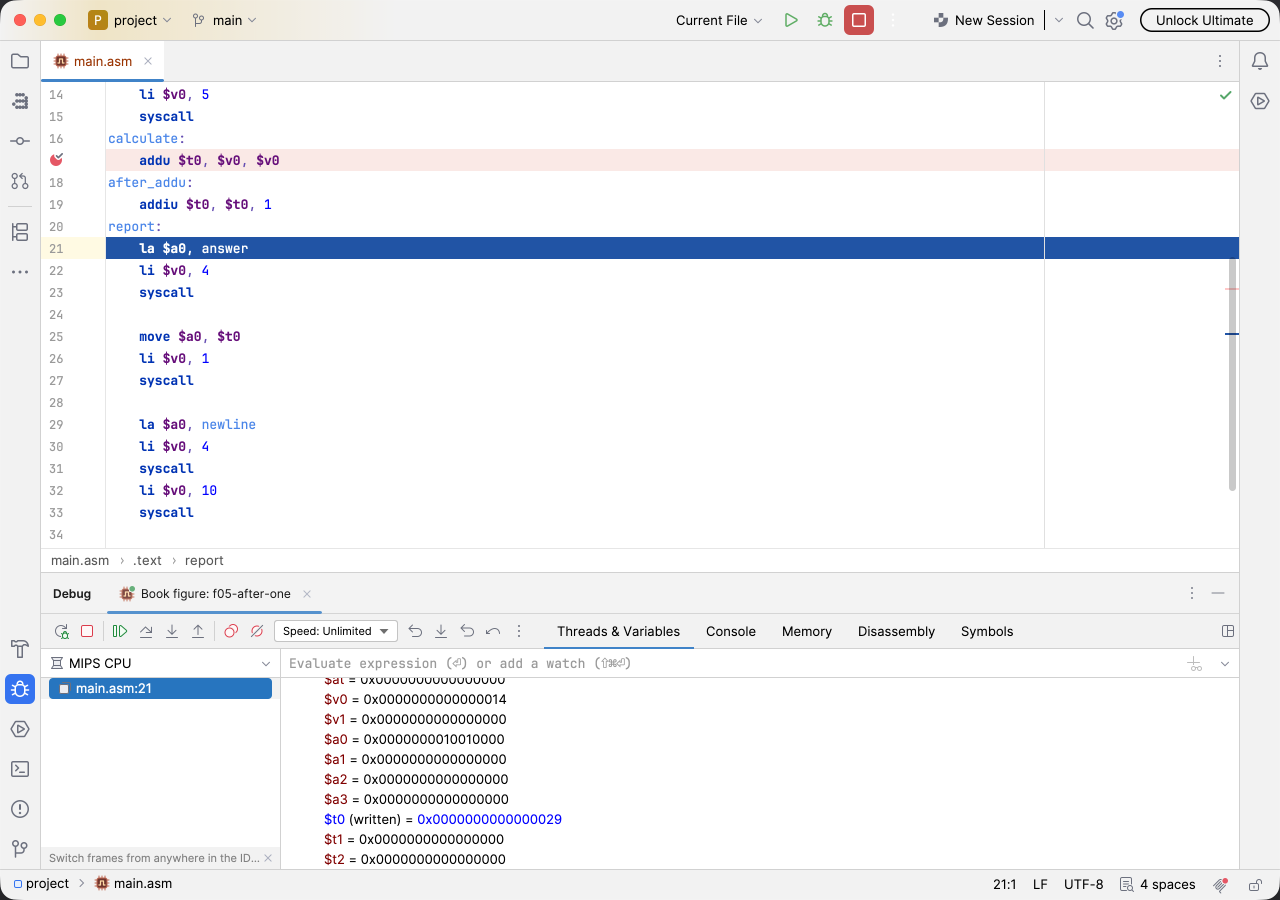
\includegraphics[width=0.53\linewidth,artifact,trim={\MARSconsoleafteronevalueLeft{} \MARSconsoleafteronevalueBottom{} \MARSconsoleafteronevalueRight{} \MARSconsoleafteronevalueTop{}},clip]{book/captures/001-console-calculation/f05-after-one/raw.png}};
\begin{scope}[shift={(value.south west)},x={($(value.south east)-(value.south west)$)},y={($(value.north west)-(value.south west)$)}]
\draw[black,line width=0.7pt] (0.023529412,0.115384615) rectangle (0.976470588,0.884615385);
\node[draw=black,fill=white,circle,inner sep=1.5pt,font=\footnotesize] at ($(0.023529412,0.884615385)+(-3mm,0)$) {2};
\end{scope}
\end{tikzpicture}
\par\smallskip
\begin{minipage}{\linewidth}
\small
\begin{enumerate}
\item The second Step Over executes \texttt{addiu}. The next \texttt{la} will form the answer-message address in \texttt{\$a0}. It does not yet print the message or copy the numeric result into the syscall argument.
\item \texttt{\$t0}=\texttt{0x29}=41. Keep this result until the reporting code moves it into \texttt{\$a0} for integer output. The following print-service selections can change \texttt{\$v0}.
\end{enumerate}
\end{minipage}
\caption{After a second native Debug step. The result is ready for the reporting sequence.}
\label{capture:001-console-calculation-f05-after-one}
\end{figure}
